\begin{table*}[t]
\caption{\textbf{Quantitative restoration results.} We report PSNR$\uparrow$ and LPIPS$\downarrow$ for image restoration on the DA3 benchmark~\cite{depthanything3}, comparing single-view and multi-view restoration approaches. The best result is highlighted in \textbf{bold} and the second best is \underline{underlined}.}
\label{tab:image_metric}
\centering
%\setlength{\tabcolsep}{3pt}
%\renewcommand{\arraystretch}{1.05}

\resizebox{\linewidth}{!}{
\begin{tabular}{lccccc ccccc ccccc ccccc}
\toprule
\multirow{2}{*}{\textbf{Model}}
& \multicolumn{2}{c}{\textbf{HiRoom}}
& \multicolumn{2}{c}{\textbf{ETH3D}}
& \multicolumn{2}{c}{\textbf{DTU}}
& \multicolumn{2}{c}{\textbf{7Scenes}}
& \multicolumn{2}{c}{\textbf{ScanNet$++$}} \\
\cmidrule(lr){2-3} \cmidrule(lr){4-5} \cmidrule(lr){6-7} \cmidrule(lr){8-9} \cmidrule(lr){10-11}

& PSNR$\uparrow$ & LPIPS$\downarrow$
& PSNR$\uparrow$ & LPIPS$\downarrow$
& PSNR$\uparrow$ & LPIPS$\downarrow$
& PSNR$\uparrow$ & LPIPS$\downarrow$
& PSNR$\uparrow$ & LPIPS$\downarrow$ \\
% \midrule

% \textit{Input Conditions} \\
% \midrule

% LQ
% &  &  &  &  &  &  &  &  &  &  \\

\midrule

\textit{Single-View Restoration} \\
\midrule
Restormer~\cite{zamir2022restormer}
& 17.49 & 0.544
& 20.97	& 0.672
& 17.73 & 0.588
& 21.30 & {0.428}
& 21.50 & 0.415  \\

HI-Diff~\cite{chen2023hierarchical}
& 17.35 & 0.551
& 20.45 & \underline{0.586}
& 17.39  & 0.591
& 19.82	& {0.428}
& 20.68 & 0.413  \\

InstructIR~\cite{conde2024high}
& 17.51 & 0.549
& 20.93	& 0.666
& 20.38 & 0.558
& 20.93 & 0.440
& 21.15 & 0.402  \\

MoCE-IR~\cite{zamfir2024complexityexperts}
& 17.69  &    0.560
& 21.00  &    0.611
&  20.38 &    0.562
&  20.60 &    0.491
&  \underline{21.19} &    0.431
\\


\midrule
\textit{Multi-View Restoration} \\
\midrule

VRT~\cite{liang2024vrt}
& 17.47  &    0.562
& 20.82  &    0.606
& 17.61  &    0.606
& 19.79  &    0.510
& 20.83  &     0.437
\\

FMA-Net~\cite{Youk_2024_CVPR}
& 17.14 &   0.551
& 20.65 &   \textbf{0.571}
& 17.13 & 0.572
& 18.84 & 0.534
& 19.98 & 0.455
\\

% MVRM$_\text{VAE}$
% VAE$_\text{MVD}$
% &  19.11 &	0.443
% &  21.25	& 0.640
% &  20.47	& 0.450
% &  21.55 &	0.417
% & 21.06 & 	0.384  \\


% MVRM$_\text{VAE (70K)}$
VAE$_\text{MVD}$
&    \underline{19.76}	&   \underline{0.493}
&     \underline{21.37}	&   0.638
&    \underline{20.54}	&  \underline{0.434}
&     \underline{21.74}	&   \underline{0.404}
&    \underline{21.19}	&  \underline{0.379} \\


\textbf{GARD (Ours)}
% \textbf{MVRM$_\text{GARD}$ (Ours)}
& \textbf{21.89}	& \textbf{0.362}
& \textbf{21.88}	& {0.635}
& \textbf{21.25} & \textbf{0.418}
& \textbf{22.67} &	\textbf{0.249}
& \textbf{22.19} & \textbf{0.345} \\

\bottomrule
\end{tabular}
}
\end{table*}
\begin{figure}[t]
  \centering
  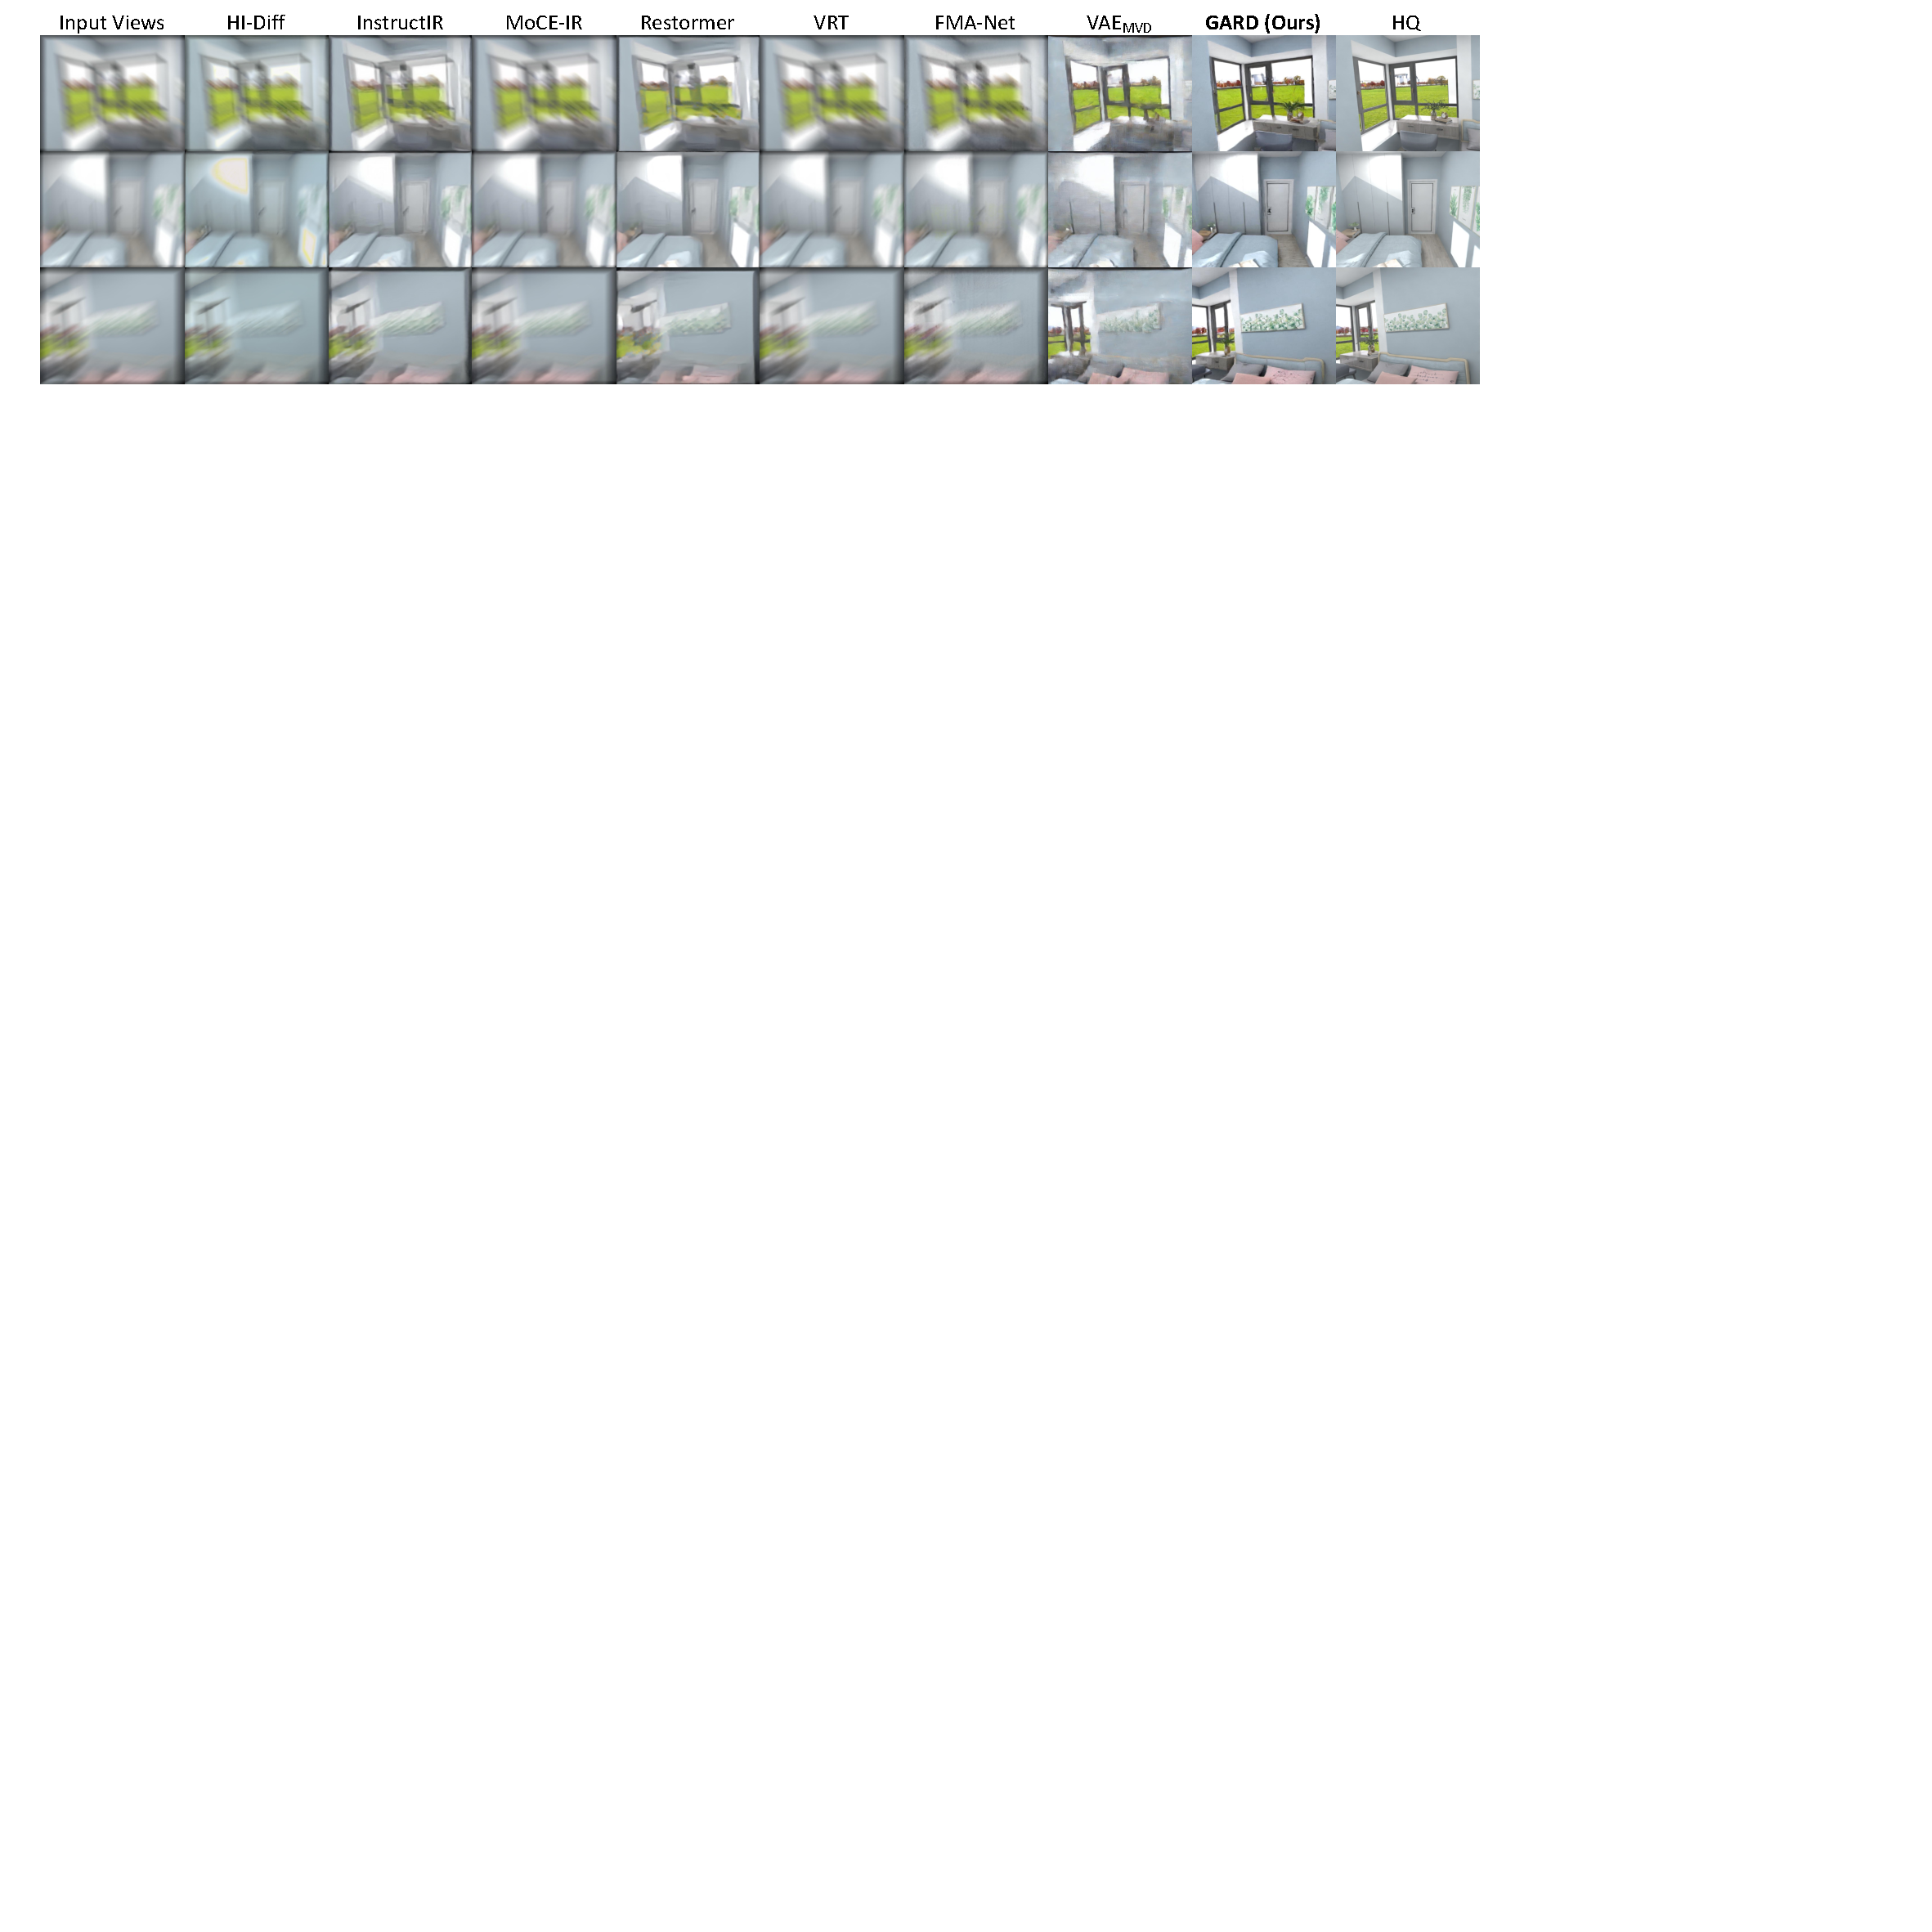
\includegraphics[width=\textwidth]{asset/rgb_main.pdf}
  \vspace{-15pt}
\caption{\textbf{Qualitative image restoration results.}
We visualize restored RGB images from degraded multi-view inputs. Compared with baseline approaches, the proposed GARD effectively recovers high-fidelity multi-view images while preserving fine-grained details. Please zoom in for clearer visualization.}
  \label{fig:rgb_main}
\end{figure}

\begin{table}[h]
\centering

\subfloat[
\textbf{Pose estimation accuracy.} We report the area under the curve (AUC30)$\uparrow$ for pose evaluation.
\label{tab:lr_ablation_pose}
]{
\begin{minipage}{0.48\linewidth}
\centering
\resizebox{\textwidth}{!}{
\begin{tabular}{lccccc}
\toprule
\multirow{2}{*}{Model} &
\multirow{2}{*}{Interp. Flow} &
\multirow{2}{*}{Alignment} &
\multicolumn{3}{c}{AUC30$\uparrow$} \\
\cmidrule(lr){4-6}
& & & ETH3D & DTU & ScanNet++ \\
\midrule
A    & \texttimes & \texttimes & 67.30 & 87.21 & 84.12 \\
B    & \texttimes & \checkmark & 66.42 & 85.49 & 84.90 \\
C    & \checkmark & \texttimes & \underline{73.85} & \underline{89.99} & \underline{85.90} \\
\midrule
D (Full) & \checkmark & \checkmark & \textbf{74.68} & \textbf{92.37} & \textbf{87.45} \\
\bottomrule
\end{tabular}}
\end{minipage}
}
\hfill
\subfloat[
\textbf{3D reconstruction accuracy.} We report Overall$\downarrow$ for DTU, while F-score$\uparrow$ is reported for the remaining benchmarks.
\label{tab:lr_ablation_recon}
]{
\begin{minipage}{0.48\linewidth}
\centering
\resizebox{\textwidth}{!}{
\begin{tabular}{lccccc}
\toprule
\multirow{2}{*}{Model} &
\multirow{2}{*}{Interp. Flow} &
\multirow{2}{*}{Alignment} &
\multicolumn{3}{c}{F-score$\uparrow$ / Overall$\downarrow$} \\
\cmidrule(lr){4-6}
& & & ETH3D & DTU & ScanNet++ \\
\midrule
A   & \texttimes & \texttimes & 39.91 & 5.43 & 31.52 \\
B    & \texttimes & \checkmark & 38.44 & 5.40 & 30.63 \\
C    & \checkmark & \texttimes & \underline{44.65} & \underline{4.92} & \underline{32.40} \\
\midrule
D (Full) & \checkmark & \checkmark & \textbf{45.79} & \textbf{4.76} & \textbf{35.77} \\
\bottomrule
\end{tabular}}
\end{minipage}
}
\vspace{-5pt}
\caption{\textbf{Ablation on GARD training components.}
We conduct an ablation study on the training components of GARD across three representative benchmarks spanning outdoor, object-centric, and indoor scenes: ETH3D~\cite{schops2017multi}, DTU~\cite{aanaes2016large}, and ScanNet++~\cite{yeshwanth2023scannet++}, respectively.}
\label{tab:abl_gard_training}\vspace{-10pt}
\end{table}



% \begin{table}[t]
% \centering
% \begin{tabular}{lcccccccc}
% \toprule
% \multirow{2}{*}{Model} &
% \multirow{2}{*}{LQ2HQ} &
% \multirow{2}{*}{Alignment} &
% \multicolumn{2}{c}{Camera Pose} &
% \multicolumn{2}{c}{3D Reconstruction} &
% \multicolumn{2}{c}{Image Metric} \\
% \cmidrule(lr){4-5}
% \cmidrule(lr){6-7}
% \cmidrule(lr){8-9}
% & &
% & Auc5$\uparrow$ & Auc30$\uparrow$
% & F-score$\uparrow$ & Acc$\uparrow$
% & PSNR$\uparrow$ & SSIM$\uparrow$ \\
% \midrule
% A    & \texttimes & \checkmark &  &  &  &  &  &  \\
% B    & \checkmark & \texttimes &  &  &  &  &  &  \\
% C    & \checkmark & \checkmark &  &  &  &  &  &  \\
% \midrule
% Full & \checkmark & \checkmark &  &  &  &  &  &  \\
% \bottomrule
% \end{tabular}
% \vspace{5pt}
% \caption{\textbf{Ablation on LQ2HQ training and attention alignment.}
% We evaluate the effects of LQ2HQ training and attention alignment on camera pose estimation, 3D reconstruction quality, and image restoration performance.}
% \label{tab:lr_ablation}
% \end{table}
\begin{table*}[h]
\centering
\subfloat[
% \textbf{Pose estimation accuracy.} Increasing the number of input views consistently improves camera pose estimation performance measured by Auc30.
\textbf{Pose estimation accuracy.} We report the area under the curve (AUC30)$\uparrow$ for pose evaluation.
\label{tab:view_ablation_a}
]{
\begin{minipage}{0.48\linewidth}
\centering
\resizebox{\textwidth}{!}{
\begin{tabular}{lccccc}
\toprule
\multirow{2}{*}{\textbf{\# Views}} &
\multicolumn{5}{c}{AUC30$\uparrow$} \\
\cmidrule(lr){2-6}
& HiRoom & ETH3D & DTU & 7Scenes & ScanNet$++$ \\
\midrule
4 views  & \underline{63.61} & 35.80 & 84.25 & 71.62 & 60.12 \\
10 views & \textbf{67.22} & 74.68 & 92.37 & 84.73 & 87.45 \\
30 views & - & \underline{82.35} & \underline{94.29}  & \underline{85.22} & \underline{94.61} \\
50 views & - & \textbf{82.62} & \textbf{98.00} & \textbf{86.85} &  \textbf{95.30} \\
\bottomrule
\end{tabular}}
\end{minipage}
}
\hfill
\subfloat[
\textbf{3D reconstruction accuracy.} We report Overall$\downarrow$ for DTU, while F-score$\uparrow$ is reported for the remaining benchmarks.
\label{tab:view_ablation_b}
]{
\begin{minipage}{0.48\linewidth}
\centering
\resizebox{\textwidth}{!}{
\begin{tabular}{lccccc}
\toprule
\multirow{2}{*}{\textbf{\# Views}} &
\multicolumn{5}{c}{F-score$\uparrow$ / Overall$\downarrow$} \\
\cmidrule(lr){2-6}
& HiRoom & ETH3D & DTU & 7Scenes & ScanNet$++$ \\
\midrule
4 views  & \underline{8.65} & 10.56 & 6.95 & 12.00 & 10.10 \\
10 views & \textbf{18.25} & 45.79 & 4.76 & 36.08 & 35.77 \\
30 views & - & \underline{58.82} & \underline{3.58} & \underline{40.47} & \underline{57.62} \\
50 views & - & \textbf{65.46} & \textbf{2.03} & \textbf{45.92} &  \textbf{65.72} \\
\bottomrule
\end{tabular}}
\end{minipage}
}
\vspace{-10pt}
\caption{\textbf{Ablation study on the number of input views.}
Increasing the number of views improves both camera pose estimation accuracy and 3D reconstruction quality, indicating that richer cross-view information substantially benefits geometric reconstruction.}
\label{tab:abl_maxview}
\vspace{-10pt}
\end{table*}

\section{Conclusion}
\label{sec:conclusion}

We presented \textbf{GARD}, a Geometry-Aware Restoration Denoising framework that performs image restoration in the geometry-aware feature space of feed-forward 3D reconstruction models. By leveraging geometry-aware representations, GARD effectively refines degraded features, which are subsequently passed to both the 3D geometry decoder and the RGB image decoder to recover accurate 3D scene geometry and high-quality restored multi-view RGB images. This representation-level denoising strategy enables the joint restoration of scene structure and appearance from degraded multi-view inputs. Extensive experiments demonstrate that GARD consistently outperforms existing single-view and multi-view restoration methods, highlighting the effectiveness of restoration in geometry-aware feature space.

\paragraph{Limitation and future directions.}
As a diffusion-based method, GARD requires iterative denoising steps, limiting its efficiency in latency-sensitive settings. Future work will focus on more efficient denoiser designs and multi-layer denoising strategies to further reduce error accumulation and improve reconstruction quality.



\clearpage